\documentclass{beamer}
\usetheme{Fulya}
%\usepackage{color}
%\usepackage[usenames,dvipsnames]{xcolor}
\usepackage{amsmath}
\usepackage{amssymb}
%\usepackage{listings}
\usepackage{tikz}
\usetikzlibrary{shapes}
\usetikzlibrary{arrows}
\usepackage{multirow}
\usepackage{rotating} %for sideways letters
\usepackage{multicol}
%\usepackage{stmaryrd} %for \llbracket (semantic bracket)
%\usepackage{lstomdoc}\lstset{language=[1.3]OMDoc,columns=fullflexible,basicstyle=\sf}
\usepackage{listings}
\usepackage{mmt_listings}
%\usepackage{xcolor}
\usepackage{../florian/basics}
\usepackage{../florian/ded}
\usepackage{../twelf-math}
\usepackage{../pattern}
\usepackage{local}




%\useoutertheme{fulyaplain}
%\setbeamertemplate{navigation symbols}{}
%\setbeamertemplate{headline}{}
%\setbeamercolor{block title}{bg=blue!50}
%\setbeamercolor{block body}{bg=blue!20}
%\setbeamertemplate{blocks}[rounded]
%
%\setbeamertemplate{footline}{
%\begin{center}\insertpagenumber\end{center}
%}
%%\lstset{mathescape,basicstyle=\footnotesize,breaklines,breakatwhitespace}
\setbeamercovered{transparent=0}
\newcommand{\lec}[1]{\strut\hfil\strut\null\nobreak\hfill\hbox{{\color{blue}#1}}\par}

\begin{document}

\title{Extending MKM Formats at the \\ Statement Level}
\author{\underline{Fulya Horozal}, Michael Kohlhase and Florian Rabe}
\institute{Jacobs University Bremen}
\date{CICM, 8.-13. July 2012 \\ Bremen, Germany}
\begin{frame}
 \titlepage
\end{frame}

\section*{Introduction}
\svnInfo $Id: intro.tex 9171 2012-03-05 08:39:33Z kohlhase $
\svnKeyword $HeadURL: https://svn.omdoc.org/repos/omdoc/projects/omdoc-2.0/pragmatic-strict/intro.tex $

The development of representation languages for mathematical knowledge is one of the
central concerns of the MKM community. After all, practical mathematical knowledge
management consists in the manipulation of expressions in such languages. To be
successful, MKM representation formats must balance multiple concerns. A format should be
expressive and flexible (for depth and ease of modeling), foundationally unconstrained
(for coverage), regular and minimal (for ease of implementation), and modular and
web-transparent (for scalability). Finally, the format should be elegant, feel natural to
mathematicians, and be easy to read and write. Needless to say that this set of
requirements is over-constrained so that the design problem for MKM representation formats
lies in relaxing some of the constraints to achieve a global optimum.

In languages for formalized mathematics, it is standard practice to define a minimal
core language that is extended by macros, functions, or notations.
For example, Isabelle \cite{isabelle} provides a rich language of notations, abbreviations, syntax and printing translations, and a number of definitional forms.
In narrative formats for mathematics, for
instance, the {\TeX/\LaTeX} format -- arguably the most commonly used format for
representing mathematical knowledge -- goes a similar way, only that the core language is
given by the {\TeX} layout primitives and the translation is realized by macro expansion
and is fully under user control. This extensibility led to the profusion of
user-defined {\LaTeX} document classes and packages that has made {\TeX/\LaTeX} so
successful.

However, the fully unconstrained nature of the extensibility makes ensuring invariants and
machine support very difficult, and thus this approach is not immediately applicable to
content markup formats. There, MathML3~\cite{CarlisleEd:MathML3:base} is a good example of
the state of the art. It specifies a core language called ``strict content MathML'' that
is equivalent to OpenMath~\cite{BusCapCar:2oms04} and ``full content MathML''. The first
subset uses a minimal set of elements representing the meaning of a mathematical
expression in a uniform, regular structure, while the second one tries to strike a
pragmatic balance between verbosity and formality. The meaning of non-strict expressions
is given by a fixed translation: the ``strict content MathML translation'' specified in
section 4.6 of the MathML3 recommendation~\cite{CarlisleEd:MathML3:base}.

This language design has the advantage that only a small, regular sublanguage has to be
given a mathematical meaning, but a larger vocabulary that is more intuitive to
practitioners of the field can be used for actual representation. Moreover, semantic
services like validation only need to be implemented for the strict subset and can be
extended to the pragmatic language by translation. Ultimately, a representation format
might even have multiple pragmatic front-ends geared towards different audiences. These
are semantically interoperable by construction.
\medskip

The work reported in this paper comes from an ongoing language design effort, where we
want to redesign our \omdoc format~\cite{Kohlhase:OMDoc1.2} into a minimal, regular core
language (\emph{strict \omdoc2}) and an extension layer (\emph{pragmatic \omdoc2}) whose
semantics is given by a ``pragmatic-to-strict'' ($\ptos$) translation.  While this problem
is well-understood for mathematical \emph{objects}, extension frameworks \emph{at the
  statement level} seem to be restricted to the non-semantic case, e.g. the
\texttt{amsthm} package for {\LaTeX}.

Languages for mathematics commonly permit a variety of pragmatic statements, e.g.,
implicit or case-based definitions, type definitions, theorems, or proof schemata.  But
representation frameworks for such languages do not include a generic mechanism that
permits introducing arbitrary pragmatic statements --- instead, a fixed set is built into
the format.  Among logical frameworks, Twelf/LF~\cite{twelf,lf} permits two statements:
defined and undefined constants. Isabelle~\cite{isabelle} and Coq~\cite{coq} permit much
larger, but still fixed sets that include, for example, recursive case-based function
definitions.  Content markup formats like \omdoc permit similar fixed sets.

A large set of statements is desirable in a representation format in order to model the
flexibility of individual languages. A large \emph{fixed} set on the other hand is
unsatisfactory because it is difficult to give a theoretical justification for fixing any
specific set of statements.  Moreover, it is often difficult to define the semantics of a
built-in statement in a foundationally unconstrained representation format because many
pragmatic statement are only meaningful under certain foundational assumptions.
%For example, an existential quantifier is needed to express the well-definedness condition of an implicit definition.
\medskip

In this paper we present a general formalism for adding new pragmatic statement forms to
our \omdoc format; we have picked \omdoc for familiarity and foundation-independence; any
other foundational format can be extended similarly. Consider for instance the pragmatic
statement of an ``implicit definition'', which defines a mathematical object by describing
it so accurately, that there is only one object that fits this description. For instance,
the exponential function $exp$ is defined as the (unique) solution of the differential
equation $f=f'$ with $f(0)=1$. This form of definition is extensively used in practical
mathematics, so pragmatic {\omdoc} should offer an infrastructure for it, whereas strict
{\omdoc} only offers ``simple definitions'' of the form $c:=d$, where $c$ is a new symbol
and $d$ any object.  In our extension framework, the $\ptos$ translation provides the
semantics of the implicit definition in terms of the strict definition $exp:=\descr
f.(f'=f\wedge f(0)=1)$, where $\descr$ is a ``definite description operator'': Given an
expression $A$ with free variable $x$, such that there is a unique $x$ that makes $A$
valid, $\descr x.A$ returns that $x$, otherwise $\descr x.A$ is undefined.

Note that the semantics of an implicit definition requires a definite description operator.
While most areas of mathematics at least implicitly assume its existence, it should not be required in general because that would prevent the representation of systems without one.
Therefore, we make these requirements explicit in a special theory that defines the new pragmatic statement and its strict semantics. This theory must be imported in order for implicit definitions to become available.
Using our extension language, we can recover a large number of existing pragmatic statements as definable special cases, including many existing ones of {\omdoc}.
Thus, when representing formal languages in {\omdoc}, authors have full control what pragmatic statements to permit and can define new ones in terms of existing ones.
\medskip

In the next section, we will recap those parts of \omdoc that are
needed in this paper. In Section~\ref{sec:pattern}, 
we define our extension language, and in Section~\ref{sec:meta}, we look at particular extensions that are motivated by mathematical practice. Finally, in Section~\ref{sec:syntax}, we will address the question
of extending the concrete syntax with pragmatic features as well.



%%% Local Variables: 
%%% mode: latex
%%% TeX-master: "paper"
%%% End: 

% LocalWords:  wrapfigure vspace hline ednote emph emph RabKoh prel Rudnicki lf
% LocalWords:  isabelle-isar aomp92 omdoc ptos frabe medskip texttt amsthm exp
% LocalWords:  descr


%\begin{frame}
%\frametitle{Outline}
%\tableofcontents
%\end{frame}

\section{Our core language}%A module system for mathematical theories}
\svnInfo $Id: mmt.tex 9195 2012-04-20 12:26:50Z frabe $
\svnKeyword $HeadURL: https://svn.omdoc.org/repos/omdoc/projects/omdoc-2.0/pragmatic-strict/mmt.tex $

\begin{wrapfigure}r{3.2cm}\vspace*{-2em}
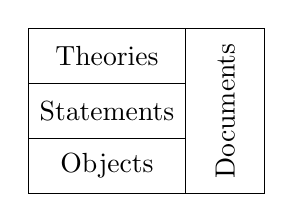
\begin{tikzpicture}[yscale=.7]
\draw (0,0) rectangle (3,3);
\draw (0,1) -- (2,1);
\draw (0,2) -- (2,2);
\draw (2,0) -- (2,3);
\node (thy) at (1,2.5) {Theories};
\node (st) at (1,1.5) {Statements};
\node (obj) at (1,0.5) {Objects};
\node (doc) at (2.5,1.5){\begin{sideways}Documents\end{sideways}};
\end{tikzpicture}
\vspace*{-2em}
\end{wrapfigure}
\omdoc is a comprehensive content-based format for representing mathematical knowledge and
documents. It represents mathematical knowledge at three levels: mathematical formulae at the
\emph{object level}, symbol declarations, definitions, notation definitions, axioms, theorems, and
proofs at the \emph{statement level}, and finally modular scopes at the \emph{theory level}. Moreover, it adds
an infrastructure for representing functional aspects of \emph{mathematical documents} at the
content markup level. \omdoc1.2 has been successfully used as a representational basis in applications
ranging from theorem prover interfaces, via knowledge based up to eLearning systems. To allow
this diversity of applications, the format has acquired a large, interconnected set of language
constructs motivated by coverage and user familiarity (i.e., by pragmatic concerns) and not by
minimality and orthogonality of language primitives (strict concerns).

To reconcile these language design issues for \omdoc2, we want to separate the format into a \emph{strict} core language
and a \emph{pragmatic} extension layer that is elaborated into strict \omdoc via a ``pragmatic-to-strict'' ($\ptos$) translation.

For strict \omdoc we employ the foundation-independent, syntactically minimal {\mmt} framework
(see below). For pragmatic \omdoc, we aim at a language that is feature-complete with
respect to \omdoc1.2~\cite{Kohlhase:OMDoc1.2}, but incorporates language features from
other MKM formats, most notably from Isabelle/Isar~\cite{isar},
PVS~\cite{pvs}, and Mizar~\cite{mizar}.

The {\mmt} language was emerged from a complete redesign of the formal core\footnote{We are currently
  working on adding an informal (natural language) representation and a non-trivial (strict)
  document level to {\mmt}, their lack does not restrict the results reported in this paper.} of \omdoc
focusing on foundation-independence, scalability, modularity, while maintaining coverage of formal
systems. The {\mmt} language is described in~\cite{RK:mmt:10} and implemented
in~\cite{project:mmt}.

\begin{wrapfigure}{l}{5.2cm}\vspace*{-2em}
\begin{center}
\begin{tikzpicture}[xscale=.95,yscale=.7]
\node[thy] (A) at (0,3)  {$\mathit{LF}$};
\node[thy] (A') at (2,3)  {$\mathit{Isabelle}$};
\node[thy] (C) at (-1,1.5)   {$\mathit{FOL}$};
\node[thy] (C') at (1,1.5) {$\mathit{HOL}$};
\node[thy] (E) at (-2,0) {$\mathit{Monoid}$};
\node[thy] (E') at (0,0)  {$\mathit{Ring}$};
\draw[meta](A) -- (C);
\draw[meta](A) -- (C');
\draw[meta](C) -- (E);
\draw[meta](C) -- (E');
\draw[struct](A) --node[above] {} (A');
\draw[struct](C) --node[above] {} (C');
\draw[struct](E) --node[above] {} (E');
%\draw[struct](A) --node[above] {$m$} (A');
%\draw[struct](C) --node[above] {$m'$} (C');
%\draw[struct](E) --node[above] {$i$} (E');
\end{tikzpicture}
\caption{An {\mmt} Theory Graph}\label{fig:mmt:intro:metatheory}
\end{center}\vspace*{-2em}
\end{wrapfigure}

MMT uses \defemph{theories} as a single primitive to represent formal systems such as logical frameworks, logics, or theories.
These form theory graphs such as the one on the left, where single arrows $\rightarrow$ denote theory translations and hooked arrows $\hookrightarrow$ denote the meta-theory relation between two theories.
The theory $\mathit{FOL}$ for first-order logic is the meta-theory for $\mathit{Monoid}$ and $\mathit{Ring}$. And the theory $\mathit{LF}$
for the logical framework LF~\cite{lf} is the meta-theory of $\mathit{FOL}$ and $\mathit{HOL}$ for higher-order logic.
In general, we describe the theories with meta-theory $M$ as \defemph{$M$-theories}.
The importance of meta-theories in {\mmt} is that the syntax and semantics of $M$ induces the syntax and semantics of all $M$-theories.
For example, if the syntax and semantics are fixed for $\mathit{LF}$, they determine those of $\mathit{FOL}$ and $\mathit{Monoid}$.

At the statement level, {\mmt} uses \defemph{constant} declarations as a single primitive to represent all OMDoc statement declarations. These are differentiated by the type system of the respective meta-theory. In particular, the Curry-Howard correspondence is used to represent axioms and theorems as plain constants (with special types).
\medskip

In Figure~\ref{fig:mmt-grammar}, we show a small fragment of the {\mmt} grammar that we need in the remainder of this paper. Meta-symbols of the BNF format are given in \bnf{color}.
%the salient language features layered according the \omdoc stratification.

%{\mmt} is meant to be applicable to all base languages based on \emph{theories}. Relations between theories (theory morphisms) are represented as {\mmt} \emph{views}. Both theories and views form the {\mmt} \emph{theory} level. A \emph{theory morphism} $\overline{\sigma} : S \rightarrow T$ is a \emph{signature morphism} $\sigma : S \rightarrow T$ interpreting all symbols of $S$ in $T$ and, in addition, $\overline{\sigma}$ translates all theorems of $S$ to theorems of $T$. {\mmt} uses the \emph{Curry-Howard representation} to drop the distinction between symbols and axioms (and thus between signatures and theories). As a result, {\mmt} needs only theories and theory morphisms.

\begin{figure}[ht]
\begin{center}
\begin{tabular}{|@{\hspace{.4em}}l@{\tb}l@{\hspace{.4em}}l@{\hspace{.4em}}l@{\hspace{.4em}}|}
\hline
Modules              & $G$      &$\bnfas$& $\bnf{(}\lfkw{theory}\;\,T = \{\Sigma\}\bnf{)^{\ast}}$\\
Theories             & $\Sigma$ &$\bnfas$& $\cdot\bnfalts\Sigma,\,%\lfkw{constant}\;\,
c \bnf{[}:E \bnf{][}=E\bnf{]}\bnfalts \lfkw{meta}\;\,T$\\   
Contexts     & $\Gamma$ &$\bnfas$& $\cdot\bnfalts\Gamma,\,x\bnf{[}:E\bnf{]}$\\ 
Expressions          & $E$      &$\bnfas$& $x\bnfalts c\bnfalts E\,E^{\bnf{+}}\bnfalts E\,\Gamma.\,E$ \\
\hline
\end{tabular}
\end{center}
\caption{{\mmt} Grammar}\label{fig:mmt-grammar}
\end{figure}

The module level of {\mmt} introduces \emph{theory declarations} $\lfkw{theory}\;\,T = \{\Sigma\}$. %\stackrel{M}{=}
Theories $\Sigma$ contain \emph{constant declarations} $c[:E_1][=E_2]$ that introduce named atomic expressions $c$ with optional type $E_1$ or definition $E_2$. Moreover, %theories can include other theories $T$ via $\lfkw{include}\;T$, and 
each theory may declare its meta-theory $T$ via $\lfkw{meta}\;T$.

{\mmt} expressions are a fragment of OpenMath~\cite{openmath} objects, for which we introduce a short syntax. They are formed from variables $x$, constants $c$, applications $E\,E_1\,\ldots\, E_n$ of functions $E$ to a sequence of arguments $E_i$, and bindings $E_1\,\Gamma.\,E_2$ that use a binder $E_1$, a context $\Gamma$ of bound variables, and a scope $E_2$.
Contexts $\Gamma$ consist of variables $x[:E]$ that can optionally attribute a type $E$.

The semantics of {\mmt} is given in terms of \emph{foundations} for the upper-most meta-theories. Foundations define in particular the typing relation between expressions, in which {\mmt} is parametric.
For example, the foundation for $\mathit{LF}$ induces the type-checking relation for all theories with meta-theory $\mathit{LF}$.

\begin{example}[{\mmt}-Theories]Below we give an {\mmt} theory $\Forms$, which will serve as the meta-theory of several logics introduced in this paper. It introduces all symbols needed to declare logical connectives and inference rules of a logic.
The syntax and semantics of this theory are defined in terms of type theory, e.g., the logical framework LF \cite{lf}.

\begin{tabular}{@{\hspace{-.55cm}}l@{\hspace{1cm}}l}
\begin{minipage}[b]{7cm}
$\kity$, $\rightarrow$, and $\lmbd$ are untyped constants representing the primitives of type theory. $\kity$ represents the universe of all types, $\rightarrow$ constructs function types $\alpha\to\beta$, and $\lmbd$ represents the $\lambda$-binder.
$\form$ is the type of logical formulas and  
%a typed constant representing the set of logical formulas. 
$\ded$ is a constant that assigns to each logical formula $F:\form$ the type $\ded\,F$ of its proof. 
\end{minipage} &
\begin{minipage}[b]{4cm}
\begin{twelfsig}
\tsig{\Forms}\\
$\kity$\\
$\rightarrow$\\
$\lmbd$\\
\decl{\form}{\kity}\\
\decl{\ded}{\form\to\kity}\\
\tsigend
\end{twelfsig}
\end{minipage}
\end{tabular}
\end{example}


%\begin{wrapfigure}{r}{4cm}
%\vspace{-3em}
%\begin{center}
%\begin{twelfsig}
%\tsig{\Forms}\\
%$\kity$\\
%$\rightarrow$\\
%$\lmbd$\\
%\decl{\form}{\kity}\\
%\decl{\ded}{\form\to\kity}\\
%\tsigend
%\end{twelfsig}
%\end{center}
%\vspace{-5em}
%\caption{An Example {\mmt} Theory}\label{fig:ex-mmt}
%\end{wrapfigure}

%{\mmt} theories consist of \emph{symbol declarations}. 
%{\mmt} views consist of \emph{symbol assignments}.  
%\emph{Constants} represent declarations of the base language.
%\emph{Structures} represent inheritance between theories.  
%\emph{Constant assignments} and \emph{structure assignments} represent assignments between constants and structures respectively. \emph{Links} are an {\mmt} module level notion that generalizes both structures and views. 
%Symbol declarations and assignments form a {\mmt} symbol level.  
%\emph{Terms} appear inside {\mmt} constants (e.g. as type or definition) and their grammar is motivated by the OpenMath grammar. They form the {\mmt} object level.


%%% Local Variables: 
%%% mode: latex
%%% TeX-master: "paper"
%%% End: 

% LocalWords:  mmt.tex wrapfigure vspace tikzpicture yscale omdoc emph Rudnicki
% LocalWords:  isabelle-isar aomp92 ednote RabKoh mmt-ontology overline hspace
% LocalWords:  rightarrow rightarrow ysep theo-name symb-name 5.2truecm xscale
% LocalWords:  cn mmt defemph frabe ptos pvs mathit hookrightarrow lf medskip
% LocalWords:  bnf hline bnfas lfkw cdot bnfalts stackrel ldots kity lmbd kity
% LocalWords:  ded ded twelfsig tsig tsigend


\section{A framework for language extensions}
\begin{frame}
\frametitle{Our Extension Layer (pragmatic OMDoc 2)}
\begin{itemize}
\item Built on top of MMT
\vspace{.5em}
\item Specify extension principles {\color{blue}{declaratively}}
\vspace{.5em}
%\item Write pragmatic features as extension schemes
%\vspace{.5em}
%\item Pragmatic language features
%\begin{itemize}
%\item defined as \alert{extension declarations}
%\item written as \alert{pragmatic declarations}
%\end{itemize}
\item Two new primitives 
\begin{itemize}
\vspace{.3em}
\item \alert{extension declarations} to {\color{blue}introduce} extension principles
\vspace{.3em}
\item \alert{pragmatic declarations} to {\color{blue}use} extension principles
\end{itemize}
\end{itemize}
%\item Defines pragmatic language features as \alert{extension}s
%\item Include extensions to write \alert{pragmatic} declarations 
\begin{block}{Syntax}
%\vspace{-.3em}
\begin{tabular}{llll}
Theories        &$\Sigma$ &$\bnfas$  & $\bnf{(}\ldots$\\[.3em]%\conDeclOp[E]{c}{E} \bnfalts \lfkw{include}\;\,T\bnfalts \lfkw{meta}\;\,T$\\
                &         &$\bnfalts$& $\extInGrammar{e}{\Lam[E_1]{x_1}\ldots\Lam[E_n]{x_n}\{\Sigma\}}$\\[.3em]
                &         &$\bnfalts$& $\pragInGrammar{c}{e\;E_1\ldots E_n}\bnf{)}^{\bnf{\ast}}$\\
%Theory families & $\Phi$  &$\bnfas$  & $\sigfr{\bnf{(}\conDeclOp[E]{c}{E}\bnf{)}^{\bnf{\ast}}}\bnfalts \pbind{x}{E}\Phi$\\ %\sigfr{\sfr}
%                & $\phi$  &$\bnfas$  & $e \bnfalts \pappl{\Phi}{E}$\\

\end{tabular}
\end{block}
\end{frame}

\begin{frame}
\frametitle{Examples}
\begin{block}{An extension principle}
\begin{twelfsig}
%\tsig{\Theorems}\\
%\tmeta{\Forms}{}\\
\tpattern{\thm}{\lflam[\form]{F}\lflam[\ded\,F]{D}}{
 \tsfdecl[D]{c}{\ded\,F}\\
}\\
%\tsigend
\end{twelfsig}
\end{block}

\begin{block}{A pragmatic declaration}
\vspace{-.3em}
\begin{twelfsig}
%\tsig{\MyTheorem}\\
%\tmeta{\Theorems}{}\\
\tpragmatic{\foo}{\thm\;(1 + 1\doteq 2)\;(\mathit{proof}\textrm{-}\mathit{term})}\\
%\tsigend
\end{twelfsig}
\end{block}
\end{frame}


\begin{frame}
\frametitle{Modularity}
\begin{block}{An extension principle}
\vspace{-.3em}
\begin{twelfsig}
\tsig{\Theorems}\\
\tmeta{\Forms}{}\\
\tpattern{\thm}{\lflam[\form]{F}\lflam[\ded\,F]{D}}{
 \tsfdecl[D]{c}{\ded\,F}\\
}\\
\tsigend
\end{twelfsig}
\vspace{-.3em}
\end{block}

\begin{block}{A pragmatic declaration}
\vspace{-.3em}
\begin{twelfsig}
\tsig{\MyTheorem}\\
\tmeta{\Theorems}{}\\
\tinclude{\mathit{Nats}}{}\\
\tpragmatic{\foo}{\thm\;(1 + 1\doteq 2)\;(\mathit{proof}\textrm{-}\mathit{term})}\\
\tsigend
\end{twelfsig}
\vspace{-.3em}
\end{block}
\end{frame}

%\begin{frame}
%\frametitle{Examples}
%\begin{block}{Implicit Definitions}
%%\begin{twelfsig}
%%\tsig{\Assertions}\\
%%\tmeta{\Forms}{}\\
%%\tpattern{\axiom}{\lflam[\form]{F}}{
%% \tsfdecl{c}{\ded\,F}\\
%%}\\
%%\tpattern{\thm}{\lflam[\form]{F}\lflam[\ded\,F]{D}}{
%% \tsfdecl[D]{c}{\ded\,F}\\
%%}\\
%%\tsigend
%%\end{twelfsig}
%%\begin{twelfsig}
%%\tsig{\Description}\\
%%\tmeta{\FOL}{}\\
%%\tpattern{\implDef}{\lflam[\term\to\form]{\psi}}{
%% \tsfdecl{p}{\term\to\term\to\term}\\
%% \tsfdecl{p_\ax}{\ded\,\forall x.\,\forall y.\,p(x,y) \Leftrightarrow \psi(x,y)}\\
%%}\\
%%\tsigend
%%\end{twelfsig}
%\begin{twelfsig}
%%\tsig{\Description}\\
%%\tmeta{\Forms}{}\\
%%\decl{\forall}{(\alpha\to\form)\to\form}\\
%%\decl{\uexists}{(\alpha\to\form)\to\form}\\
%\multicolumn{4}{@{\tb}l}{$\lfkw{extension}\;\implDef\;\tequal\;\lflam[\kity]{\alpha}\lflam[\kity]{\beta}$}\\
%\multicolumn{4}{@{\tb\;\;\;}l}{$\lflam[\alpha\to\beta\to\form]{\psi}$}\\
%\multicolumn{4}{@{\tb\;\;\;}l}{$\lflam[\ded\,\forall x\,\uexists y\mmtdot\psi\mmtpar{x\mmtcomma y}]{\welldefn}\,\clrb{\{}$}\\
%\multicolumn{4}{@{\tb\tb}l}{
%\begin{tabular}{lll}
%\tsfdecl{f}{\alpha\to\beta}\\
%\tsfdecl{\ax}{\ded\,\forall x\mmtdot \psi\mmtpar{x\mmtcomma f\mmtpar{x}}}\\
%\end{tabular}}\\
%$\clrb{\}}$
%%\tsigend
%\end{twelfsig}
%\end{block}
%
%\begin{block}{A Pragmatic Declaration}
%\begin{twelfsig}
%%\tsig{\Sqrt}\\
%%\tmeta{\FOL}{}\\
%%\tmeta{\Description}{}\\
%%\decl{\nat}{\kity}\\
%%\decl{\real}{\kity}\\
%%$\vdots$\\%\decl{\caret}{\kity}\\
%\tpragmatic{\sqrt{}}{\implDef\;\nat\;\real\;(\lmbd\,r.\,\lmbd\,n.\,r^2 = n\;\wedge\;r\geq 0)\;(\ded\ldots)}\\
%%(\lflam[\nat]{n}\lflam[\real]{r} r^2\doteq n\;\wedge\;r\geq 0)\;(\ded\ldots)}\\
%%\tsigend
%\end{twelfsig}
%\end{block}
%
%%$\psi$ denotes an MMT term representing $r^2 = n\;\wedge\;r\geq 0$\\ for $r\in\Real$ and $n\in\Nat$.
%%\begin{block}{}%{Pragmatic Declarations}
%%\vspace{-.3em}
%%%\begin{itemize}
%%%\item 
%%Extension $\implDef$ permits pragmatic declarations of the form
%%\vspace{-.5em}
%%\center{$\pragmatic{c}{\implDef\;\alpha\,\beta\,\psi}$.}
%%%{\color{blue}$f : \implDef\;\alpha\,\beta\,\psi$}.
%%%\item E.g., $\sqrt : \implDef$
%%%%\item Extension $\thm$ permits {\color{blue}$c : \thm\;F\;D$}.
%%%\end{itemize}
%%\end{block}
%\end{frame}


%\begin{frame}
%\frametitle{Example}
%\begin{block}{Pragmatic Declarations}
%\begin{twelfsig}
%\tsig{\Sqrt}\\
%\tmeta{\FOL}{}\\
%\tmeta{\Description}{}\\
%\decl{\nat}{\kity}\\
%\decl{\real}{\kity}\\
%$\vdots$\\%\decl{\caret}{\kity}\\
%\tpragmatic{\sqrt{}}{\implDef\;\nat\;\real\;\psi\;(\ded\ldots)}\\
%%(\lflam[\nat]{n}\lflam[\real]{r} r^2\doteq n\;\wedge\;r\geq 0)\;(\ded\ldots)}\\
%\tsigend
%\end{twelfsig}
%\end{block}
%
%$\psi$ denotes an MMT term representing $r^2 = n\;\wedge\;r\geq 0$.
%\end{frame}


\begin{frame}
\frametitle{Pragmatic-to-Strict Translation}
Semantics of pragmatic declarations:\\
Elaborate pragmatic declarations into strict (core) declarations.

\begin{block}{}
\vspace{-.3em}
\begin{twelfsig}
\multicolumn{4}{@{\tb}l}{$\lfkw{extension}\;e\;\tequal\;\lflam[E_1]{x_1}\ldots\lflam[E_n]{x_n}\clrb{\{}$}\\
\multicolumn{4}{@{\tb\tb}l}{
\begin{tabular}{lll}
\tsfdecl[D_1]{c_1}{\tau_1}\\
$\vdots$\\
\tsfdecl[D_n]{c_n}{\tau_n}\\
\end{tabular}}\\
$\clrb{\}}$
\\
\tpragmatic{p}{e\;A_1\ldots\;A_n}
\end{twelfsig}
\vspace{-.3em}
\end{block}

%\begin{flushleft}
\begin{tikzpicture}
%\node(p) at (5,3) {
\node(p) at (-4,.6) {
\begin{twelfsig}
\decl{p}{e\;A_1\ldots\;A_n}
\end{twelfsig}
};

\node(c1) at (3,1) {$p\mmtdot c_1\mmtcolon\gamma(\tau_1)\;\tequal\;\gamma(D_1)$};
\node(m) at (3,.6) {$\vdots$};
\node(cn) at (3,0) {$p\mmtdot c_n\mmtcolon\gamma(\tau_n)\;\tequal\;\gamma(D_n)$};
\draw[blue,-\arrowtip] (p) --node[above] {elaborate} (.8,.6);
\end{tikzpicture}
%\end{flushleft}

$\gamma$ substitutes $A_i$ for $x_i$ and $p.c_i$ for $c_i$.
%\end{center}

%\begin{block}{}
%\vspace{-.6em}
%\begin{twelfsig}
%\tpragmatic{p}{e\;A_1\ldots\;A_n}
%\end{twelfsig}
%\end{block}
%
%\begin{center}
%\begin{tikzpicture}
%\node(c)  at (0,.5) {$p$};
%\node(c1) at (5,1) {$p\mmtdot c_1\mmtcolon\gamma(\tau_1)\;\tequal\;\gamma(D_1)$};
%\node(m) at (5,.6) {$\vdots$};
%\node(cn) at (5,0) {$p\mmtdot c_n\mmtcolon\gamma(\tau_n)\;\tequal\;\gamma(D_n)$};
%\draw[blue,->] (c) --node[above] {elaborate} (3,.5);
%\end{tikzpicture}
%\end{center}


%Elaborate pragmatic declaration 
%\[\pragmatic{c}{e\,E_1\,\ldots\,E_n}\]
%to a list of strict declarations
%\[
%c\mmtdot d_1\mmtcolon \gamma(D_1)\mmteq\gamma(D_1)
%\]
%\begin{tikzpicture}
%\node at (0,4) {$\pragmatic{c}{e\,E_1\,\ldots\,E_n}$};
%\node at (0,3) {$\conDecl{\mmtdot{c}{d_1}}{\Gamma{}}$};
%\end{tikzpicture}
\end{frame}


\begin{frame}
\frametitle{Various Extension Principles}
%\only<1>{
%\begin{block}{Implicit Definitions in OMDoc}
%\begin{twelfsig}
%\tsig{\Description}\\
%\tmeta{\Forms}{}\\
%\decl{\uexists}{(\alpha\to\form)\to\form}\\
%\decl{\descr}{(\alpha\to\form)\to\alpha}\\
%\decl{\descr_{\ax}}{\ded\,\uexists x\,P\,x\to \ded\,P\,(\descr\,P)}\\
%[.5em]
%\tpattern{\implDef}{\lflam[\kity]{\alpha}\lflam[\alpha\to\form]{P}\lflam[\ded\,\uexists x:\alpha.\,P\,x]{m}}{
% \tsfdecl{c}{\alpha\;\;=\;\;\descr\,P}\\
% \tsfdecl{c_\ax}{\ded\,\uexists x:\alpha.\,P\,x}\\
%}\\
%\tsigend
%\end{twelfsig}
%\end{block}
%}
\only<1>{
\begin{block}{Mizar-Style Functor Definitions}
\begin{twelfsig}
\tsig{\FunctorDefinitions}\\
\tmeta{\Forms}{}\\
%$\vdots$\\
%\decl{\wedge}{\form\to\form\to\form}\\
%\decl{\impl}{\form\to\form\to\form}\\
%\decl{\forall}{(\alpha\to\form)\to\alpha}\\
%\decl{\exists}{(\alpha\to\form)\to\alpha}\\
%\decl{\eqn}{\alpha\to\alpha\to\form}\\
\multicolumn{4}{@{\tb}l}{$\lfkw{extension}\;\functor\;=\lflam[\kity]{\alpha}\lflam[\kity]{\beta}$}\\
\multicolumn{4}{@{\tb\;\;\;}l}{$\lflam[\alpha\to\beta\to\form]{\means}\lflam[\ded\ldots]{\existence}$}\\
\multicolumn{4}{@{\tb\;\;\;}l}{$\lflam[\ded\ldots]{\uniqueness}\,\clrb{\{}$}\\
\multicolumn{4}{@{\tb\tb}l}{
\begin{tabular}{lll}
\tsfdecl{f}{\alpha\to\beta}\\
\tsfdecl{\defthm}{\ded\,\forall x\mmtcolon\alpha\mmtdot\,\means\,x\,\mmtpar{f\,x}}\\
\end{tabular}}\\
$\clrb{\}}$\\
\tsigend
\end{twelfsig}
\end{block}

%\begin{block}{$\pragmatic{F}{\functor\;\alpha\;\beta\;P\;\rho_1\;\rho_2}$}%Pragmatic Declaration}
%\vspace{-.5em}
%%
%\end{block}
}
\only<2>{
\begin{block}{HOL-Style Type Definitions}
\begin{twelfsig}
\tsig{\Types}\\
\tmeta{\Forms}{}\\
%$\vdots$\\
%\decl{\forall}{(\alpha\to\form)\to\form}\\
%\decl{\exists}{(\alpha\to\form)\to\form}\\
%\decl{\doteq}{(\alpha\to\alpha)\to\form}\\
\tpattern{\typeDef}{\lflam[\kity]{\alpha}\lflam[\alpha\to\form]{A}\lflam[\ded\ldots]{\rho}}{ %[\ded\,\exists x:\alpha.\,A\,x]
 \tsfdecl{T}{\kity}\\
 \tsfdecl{\Rep}{T\to\alpha}\\
 \tsfdecl{\Abs}{\alpha\to T}\\
 \tsfdecl{{\Rep'}}{\ded\,\forall x\mmtcolon T\mmtdot\,A\,\mmtpar{\Rep\,x}}\\
 \tsfdecl{{\RepInv}}{\ded\,\forall x\mmtcolon T\mmtdot\,\Abs\,\mmtpar{\Rep\,x} \doteq x}\\
 \tsfdecl{{\AbsInv}}{\ded\,\forall x\mmtcolon\alpha\mmtdot\,A\,x\impl\Rep\,\mmtpar{\Abs\,x} \doteq x}\\
}\\
\tsigend
\end{twelfsig}
\end{block}

%\begin{block}{$\pragmatic{t}{\typeDef\;\alpha\,A\,\rho}$}
%\vspace{-.5em}
%\end{block}

%$\rho$ denotes a proof for the non-emptiness of $A$.
}
%\only<3>{
%\begin{block}{Case-Based Definitions}
%\begin{twelfsig}
%\tsig{\CaseBased}\\
%\tmeta{\Forms}{}\\
%%$\wedge$\\
%%$\impl$\\
%%$\forall$\\
%%\decl{\wedge}{\form^n\to\form}\\
%%\decl{\vee^{!}}{\form^n\to\form}\\
%%\decl{\impl}{\form\to\form\to\form}\\
%%\decl{\forall}{(\alpha\to\form)\to\form}\\
%\multicolumn{4}{@{\tb}l}{$\lfkw{extension}\;\casedef\;=\;\lflam[\mathbb{N}]{n}\lflam[\kity]{\alpha}\lflam[\kity]{\beta}\lflam[(\alpha\to\form)^n]{c}$}\\
%& &$\hspace{2.65cm}\lflam[(\alpha\to\beta)^n]{d}\lflam[\ded\,\forall x:\alpha.\, \vee^{!} \lfseqbind{c_i\,x}{i}{n}]{\rho}\{$ \\
%\multicolumn{4}{@{\tb\tb}l}{
%\begin{tabular}{lll}
%\tsfdecl{f}{\alpha\to\beta}\\
%$\ax$ & $:$ &$\ded\,\forall x:\alpha.\,\wedge\,\lfseqbind{c_i\,x\,\impl\,(f\,x) = (d_i\,x)}{i}{n}$\\
%\end{tabular}}\\
%\multicolumn{4}{@{\tb}l}{$\}$}\\
%%\tpattern{\caseBasedDef}{\lflam[\mathbb{N}]{n}\lflam[\kity]{\alpha}\lflam[\kity]{\beta}\lflam[(\alpha\to\form)^n]{c}\lflam[(\alpha\to\beta)^n]{d}\lflam[\ded\,\forall x:\alpha.\, \vee^{!} \lfseqbind{c_i\,x}{i}{n}]{m}}{
%% \tsfdecl{f}{\alpha\to\beta}\\
%% \tsfdecl{\ax}{\ded\,\forall x:\alpha.\,\wedge\,\lfseqbind{c_i\,x\,\impl\,(f\,x) = (d_i\,x)}{i}{n}}\\ 
%%}\\
%\tsigend
%\end{twelfsig}
%\end{block}
%}
\end{frame}


\section{Concrete syntax} %Syntax extensions and surface language}
\begin{frame}[fragile]
\frametitle{Concrete Syntax for Our Extension Layer}
\begin{itemize}
\item For bidirectional pragmatic-to-strict translation
\item $\extension{e}{\lflam[E_1]{x_1}\ldots\lflam[E_n]{x_n}\sigfr{\Sigma}}$ is written as 

%\begin{block}{}
%\vspace{-.5em}
\begin{center}
\begin{lstlisting}
<extension name="$e$">
 <parameter name="$x_1$">$E_1$</parameter>
  $\hspace{2cm}\vdots$
  <parameter name="$x_n$">$E_n$</parameter>
  <theory>
      $\Sigma$
  </theory>
</extension>
\end{lstlisting}
\end{center}
%\end{block}
\vspace{.5em}
\item $\pragmatic{c}{e\;A_1\ldots A_n}$ is written as 
%\begin{block}{}
%\vspace{-.5em}
\begin{center}
\begin{lstlisting}
<pragmatic name="$c$" extension="$\mmturi{e}$">
    $A_1\ldots A_n$
</pragmatic>
\end{lstlisting}
\end{center}
%\end{block}

{\footnotesize $\mmturi{e}$ denotes $e$'s URI.}
\end{itemize}
\end{frame}

%\llquote{M}
%$\om{E_1}\ldots\om{E_n}$
%$\hspace{.45cm}\om{\Sigma}$
%<parameter name="$x_1$">$\om{E_1}$</parameter>


\begin{frame}
\frametitle{Pragmatic Surface Syntax}
\begin{itemize}
%\item A human-oriented syntax closer to notational convensions
\item Notation parser specific to each pragmatic surface syntax 
\lec{ongoing work for our Twelf surface syntax}
\lec{done for our sTeX surface syntax}
\end{itemize}

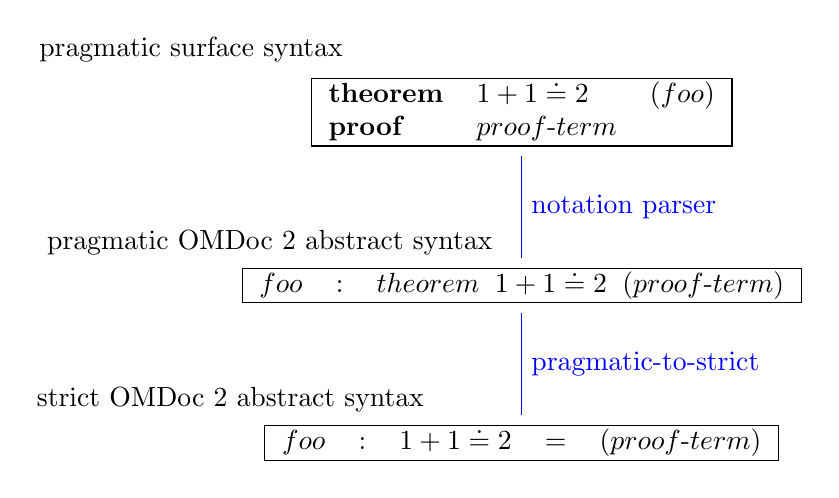
\begin{tikzpicture}
\node(n) at (4,4.2) {
\begin{tabular}{|lll|}\hline
\textbf{theorem} & $1 + 1 \doteq 2$ & $(foo)$ \\
\textbf{proof}   & $proof\textrm{-}term$ &\\
\hline
\end{tabular}
};

\node at (-.2,5) {\alert{pragmatic surface syntax}};
\node at (.8,2.55) {\alert{pragmatic OMDoc 2 abstract syntax}};
\node at (.3,.55) {\alert{strict OMDoc 2 abstract syntax}};
\node(p) at (4,2) {
\begin{tabular}{|lll|}\hline
$foo$ &:& $theorem\;\;1 + 1 \doteq 2\;\;(proof\textrm{-}term)$\\\hline
\end{tabular}
};

\node(s) at (4,0) {
\begin{tabular}{|lllll|}\hline
$foo$ &:& $1 + 1 \doteq 2$ &=& $(proof\textrm{-}term)$\\\hline
\end{tabular}
};

\draw[blue,-\arrowtip] (n) --node[right] {notation parser} (p);
\draw[blue,-\arrowtip] (p) --node[right] {pragmatic-to-strict} (s);
\end{tikzpicture}
%\begin{tabular}{|lll|}\hline
%\textbf{theorem} & $1 + 1 \doteq 2$ & (foo) \\
%\textbf{proof}   & proof-term &\\
%\hline
%\end{tabular}
\end{frame}

\section*{Summary}
\begin{frame}
\frametitle{Conclusion and Future Work}
\begin{itemize}
\item User-definable, constrained, statement level extensions in MKM formats
\item Generic: applicable to virtually any declarative language
\item Realized within the OMDoc/MMT language
\item Expressed common conservative extension principles 
\item Future: test with extension principles from widely used MKM formats %to find limitations
\begin{itemize}
\item create library of extension principles
\item find limitations (candidates: abstract data types, proof schemas)
\end{itemize}
\end{itemize}
\end{frame}



\end{document}

\begin{frame}
\frametitle{}
\begin{itemize}
\item 
\item 
\end{itemize}
\end{frame}

\begin{frame}
\frametitle{test}
\begin{itemize}
\onslide<1>{
\item A
}
\onslide<2>{
\item B
}


